\documentclass[a4paper,11pt]{article}
\usepackage[british]{babel}
\usepackage[top=1.5cm,bottom=1.5cm,left=1.5cm,right=1.5cm]{geometry}
\usepackage{graphicx}
\usepackage[hyphens]{url}
\usepackage{paralist}
\usepackage{authblk}
\usepackage[noadjust]{cite}
\usepackage[pdftex,colorlinks=true]{hyperref}


% title
\title{Facilitating Collaborative Learning Between Remote Sites}

% names
\author[1]{James McNaughton}
\author[2]{Tom Crick}
% \author[3]{}
% \author[4]{}
% \author[5]{}
% affiliation
\affil[1]{School of Education, Durham University, UK} % Need to check this.
\affil[2]{Department of Computing \& Information Systems, Cardiff
  Metropolitan University, UK}
% \affil[3]{}
% \affil[4]{}
% \affil[5]{}
% emails
\affil[1]{\protect\url{j.a.mcnaughton@durham.ac.uk}}
\affil[2]{\protect\url{tcrick@cardiffmet.ac.uk}}
% \affil[3]{\protect\url{}}
% \affil[4]{\protect\url{}}
% \affil[5]{\protect\url{}}

\renewcommand\Authands{ and }
\def\UrlBreaks{\do\/\do-}

\date{ }

\begin{document}
\maketitle


\begin{abstract}
This work details a study in the use of large touch-screen interfaces to facilitate collaborative education between students at separate locations, specifically the North East of England and South Wales.
An app for supporting a collaborative classroom activity was created for this study which allowed students at either location to transfer materials to the students at the other locations via a `flick' gesture.
The execution of the trial required several novel innovations to overcome shortcomings with the app's supporting framework and the technologies used.
With data collected from the successful completion of the trial a thorough approach has now been outlined for its analysis.
\end{abstract}

% Using JORS-friendly structure
\section{Introduction}

Large touch screen interfaces offer many opportunities for collaboration between co-located users. % refs
Not just when the interface is shared but when two or more co-located interfaces are networked together to allow for the transfer of materials between them. % refs
There are many benefits to collaborating with configurations of interfaces like this, especially in education settings. % refs
In the past there have been several studies investigating the impact of these configuration on KS2 and 3 classrooms. % More on education + collaborative education impact of touchscreens?

Previous studies have been concerned with how the use of multiple large touch screen interfaces impacts on collaborative education in single environments, i.e. Individual classrooms. % refs
However, with the opportunities afforded by large networks, such as the internet, for collaboration in education across multiple locations [refs], the limitations of co-located interfaces become much more apparent.
One of the key advantages of collaborative education across multiple locations is that it allows students with a potentially much wider range of backgrounds and skills to work together. % refs

This work details a study that was designed around investigating the impact of applying the use of large touch screen interfaces to multiple separate locations, specifically KS1/2/3? classrooms, on collaborate education. % Which key stage were the participants?

The use of a touch screen interface offers the opportunity for many novel gestures to intuitively instigate specific actions. % refs
One such gesture is the flick motion~\cite{reetz-et-al:2006} which is typically used for the movement of materials about an environment with minimal effort.
This gesture benefits collaboration greatly, allowing users to transfer materials to each other without needing to enter each other's interaction space.
 
It is possible that the flick gesture could be used, not only for passing content between users on the same interface, but for passing materials to users on remote interfaces.
This study builds on this possibility and applies it to the transferral of materials between non-co-located locations.

\subsection{Theoretical groundings}

% Todo

\subsection{Literature}

% Todo


\section{SynergyNet}

It was decided that the SynergyNet~\cite{alagha-et-al:2010,higgins-et-al:2011} framework would be used as part of this study as it is built specifically for supporting applications intended to be used in education.
SynergyNet allows for applications (apps) built with the framework to apply gesture listeners to any content items they contain.
This has the result of allowing any content item supported by the framework to be moved and manipulated by users through common multi-touch gestures.

There are two main versions of the framework; SynergyNet 2 and SynergyNet 3.
The big difference between these two frameworks is that a lot of the functionality is supplied at a framework level in SynergyNet 3 rather than at an app level as it was in SynergyNet 2.
For the remainder of this work any references to the SynergyNet framework relate to SynergyNet 3 unless stated otherwise.

The framework supports many features beyond its ability to be used with multiple multi-touch technologies.
One such feature is its ability to support communication between multiple interfaces via a network connection.
This use of networked interfaces allows media-based content to be easily shared between multiple users.
The framework supports several different methods to transfer materials between instances of its apps.
In apps used in previous studies, control over the transfer of materials has been given to the teacher who uses a separate interface to instigate the transferral of content. % refs

% Education impact of SynergyNet in the past.

\subsection{Network Flick}

SynergyNet's support for multi-touch interface allows users to perform a flicking~\cite{reetz-et-al:2006} motion to transfer content.
This gesture is built on the metaphor of pushing items around on a low-friction surface (like ice) where a small amount of initial effort can allow the item the force is exerted on to travel a great distance.
An amount of friction can be applied to decelerate flicked objects over time which is useful for both helping users keep control of items (i.e.
so they don't travel indefinitely at high speeds after being flicked making them difficult to grab and stop) and for making the behaviour of the item better match its real world equivalent from the metaphor of objects on ice.

The networking element of this gesture comes when users flick a content item in the direction of the interface they wish to send content to.
The item travels off the side of the initial interface and appears on the target interface as shown in Figure~\ref{fig:FlickExample}.
Flicking in a direction where there is no interface results in the item bouncing off the interface boundary.

\begin{figure}[h]
 \centering
   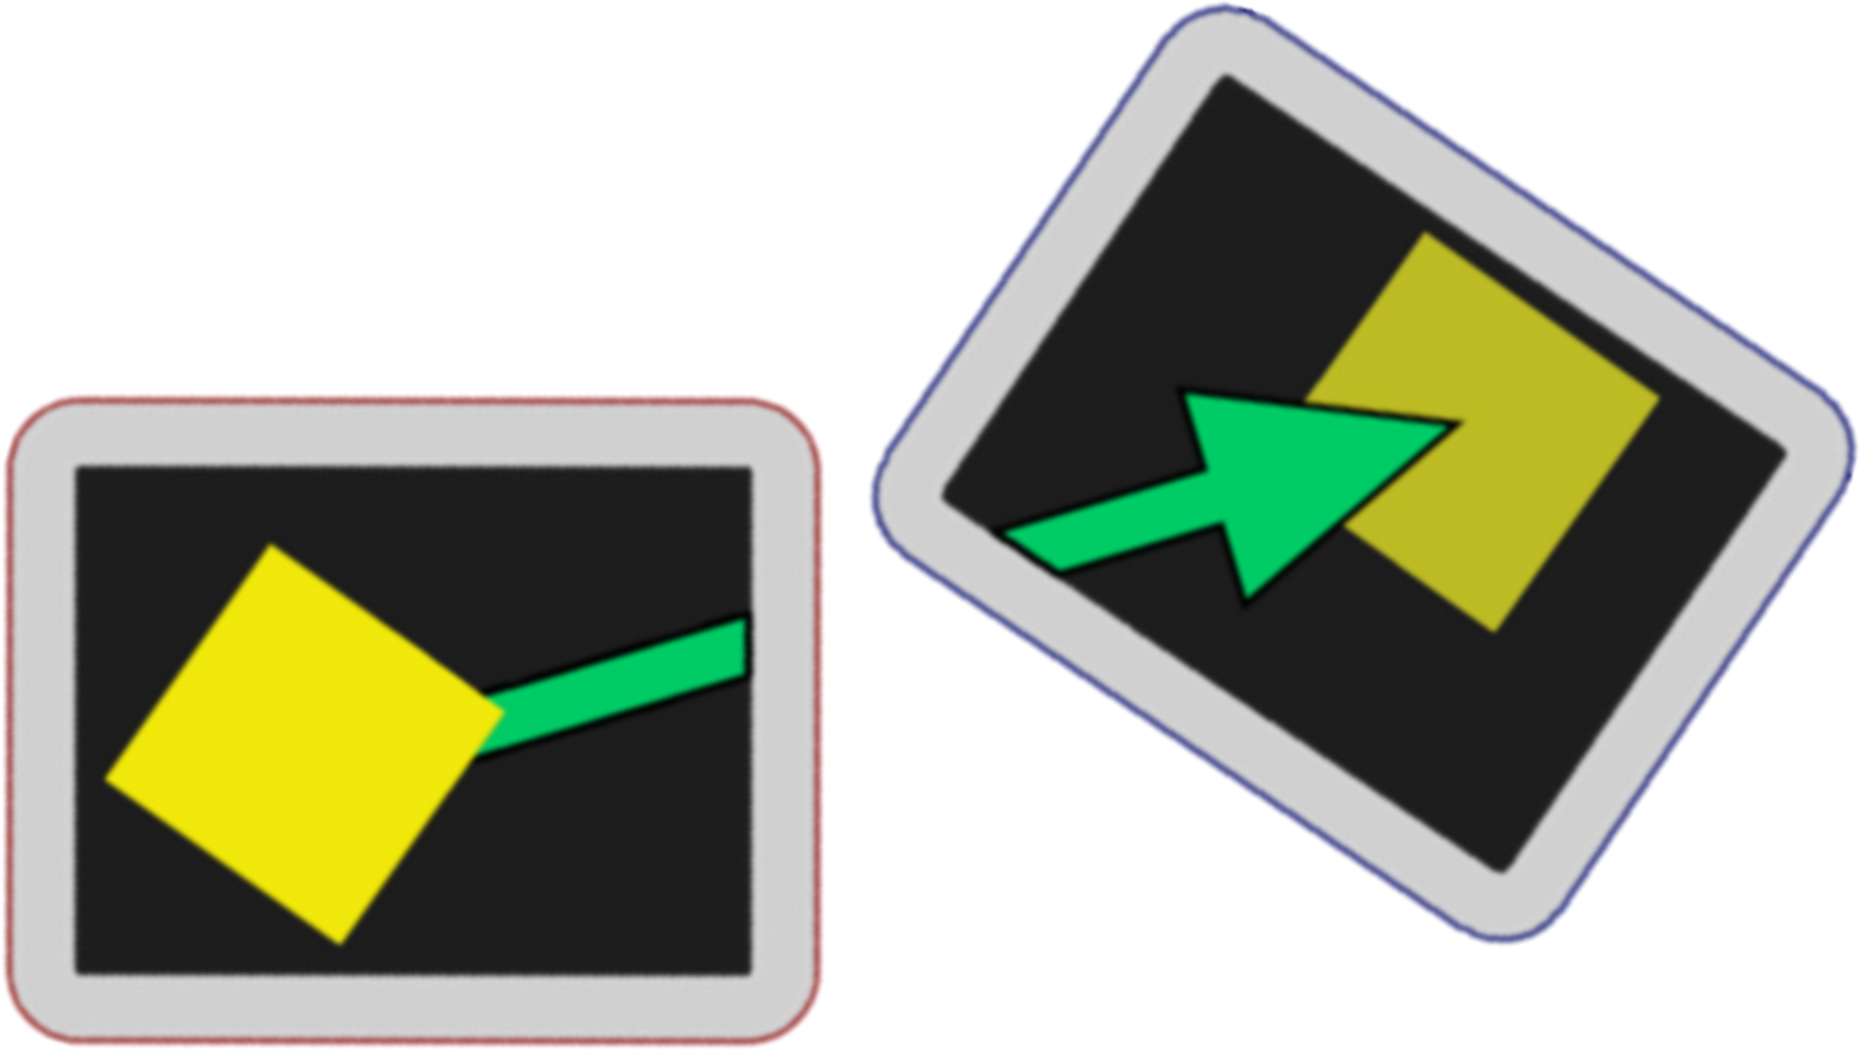
\includegraphics[width=0.75\textwidth]{figures/flickexample.png}
   \caption{The use of the network flick gesture to transfer content between co-located interfaces.}
   \label{fig:FlickExample}
\end{figure}

When the item arrives on the target interface, the framework can use its knowledge of the interface locations to ensure the item travels into view from the direction of the source interface.
This is intended to aid users in identifying where newly arrived content items were sent from when the interfaces are co-located.

The use of a flicking gesture not only informs users on recipient interfaces of the genesis of transferred items but also creates an intuitive way of sending content.
Users are capable of choosing their recipient through the direction of the flick and start the transfer simply by moving the item in that direction and releasing it.
This is intended to reduce the cognitive load usually required to move content between interfaces.
The potential benefit is thought to be that by having a simple method to move content between interfaces, users will be more willing to share items as there is less of a barrier to sending and receiving.

Though the network flick gesture is attention grabbing, little use has been found for it.
The feature has been present in The SynergyNet framework since its earliest versions but very few apps utilise it.
While some apps that entail the transfer of materials between interfaces do support the gesture, most encourage users to use other, more traditional, methods of sharing contents (such as placing items in shared areas or through using a context menu).

Some previous studies have been carried out investigating the HCI-aspects of the network flick gesture [papers in progress] but none of these have entailed its use in a classroom environment.
Typically, classroom-based studies with SynergyNet have utilised a remote teacher interface to orchestrate the transferal of content. % refs

Though the gesture is often used in the warm-up and cool-down sessions (to get participants used to interacting through the touch-screens and as a form of reward respectively) during previous studies with KS 1 and 2 students and has always been well received, there has been little data collected on its use by pupils as part of classroom activities.
Where it has been used, the network flick has always been performed to transfer content between two co-located interfaces previously.

\subsection{Co-Location}

The majority of SynergyNet features have been developed with co-located interfaces as the intended environment for their use.
Often in the past, the apps developed for SynergyNet and features for the framework itself have been created for specific studies.
As all of these studies took place in singular environments the features and apps of the framework were built assuming co-located environments.
Though efforts were made to ensure that SynergyNet was dynamic and adaptable as possible, functioning across multiple environments in separate locations was not a priority during its past development and as a consequence there are several shortcoming in the systems.
This is apparent in both the visual and functional design of the framework and apps.

Many of the interfaces presume that users will be together in the same environment and able to see each other's screen directly.
This has a large impact on the design of visual elements, such as menus.
For example, the menu used by teachers to transfer content in previous studies assumes that the teacher is able to see pupil's interfaces so that they can choose which group's work they can display to the class.

% Could add a bit here about the use of the Kinect and table selection through pointing in the last SynergyNet studies but maybe best not to muddy the waters.

The network flick gesture makes a large presumption about its use which results from its intention for use between co-located interfaces.
This is that users will know where their target interface is in relation to them.
However, this knowledge can be made available to users even when their target interface is in a remote location.
The implications of not directly seeing the target interface when performing a network flick gesture are one of the focuses of this study.

\subsection{Other Technical Considerations}

Not only has the design of the SynergyNet framework and its apps been limited by the assumption of use across only co-located interfaces.
The technical workings of the system have also been restricted.
The use of single environments in the past meant that the framework was always deployed across a single Local Area Network LAN) in all studies.
As there was no need previously for the framework to be able to work across anything beyond a LAN many of the features are not capable of functioning across the internet.

Despite the intention of being used solely across LANs in the past a large amount of the framework's networking capability was built in such a way that it could function across the internet.
The use of third party libraries such as OpenFire * and Hazelcast * mean that the framework can use several different protocols across wider networks for communicating messages to each other. %refs

However, there are some network features that are limited to LAN.
An example of this is how media content is transferred between instances of the framework.
The framework uses a shared network location as a form of cache.
This was beneficial in the past as it was simple to implement and gave teachers a single location to collect the files used in a study session from for use in future lessons.
The secure use of a shared network location across a wider network, such as the internet, is inadvisable without precautions due to the security and speed of such a technique.
It was therefore a requirement that some development work took place prior to this work's study taking place to allow the framework, or at least the app used, to function over the internet as the two locations used would not be able to share a typical LAN.

% need to have a focus on the software...


\section{Pilot Study}

For the study, two groups of KS1 students at separate locations were encouraged to work together on a classroom activity. % Need to double check the key stage of the students.
One group were situated in a school in the North East of England and the other in a school in South Wales.
Each group was allocated a large touch-screen interface to work together on the activity with.
Touch-screen table-top interfaces (Samsung SUR40s) were used.
The horizontal nature of the interfaces was chosen to allow multiple students to work around the devices.
The two table-top interfaces were networked together to share content between them, specifically through the network flick gesture.
To allow the teams to communicate and to give them a direction to focus their flick gestures towards, a tablet was positioned by the tables along one side at both locations.
This tablet used video-conference software (i.e.
Skype) to allow the teams to see each other.
The tables were configured so that flicking items towards the tablet screen would transfer them to the remote table.
This was achieved by configuring the tables so that they were virtually positioned next to each other (with the sides on which the tablets were placed being parallel to each other) when in reality they were on opposite sides of the country.
This meant each table considered the other to be co-located.
With students passing items towards their `window' to the other team, the metaphor of physically pushing items towards another interfaces was maintained.

Virtually positioning the tables side-by-side also meant that the entire edge of the tables with the tablet on (one of the longer edges of the widescreen aspect ratio interfaces) could be used as the target for network flicks.
If the two tables were configured to use their real-life locations in relation to each other, the size of the boundary where a network flick could be trigged (i.e.
that points to the remote table) would be less than a pixel at the distance between the two locations.

Another benefit to this configuration of the tables being placed virtual side-by-side relates to the behaviour of the transfer.
Normally a realistic effect is employed where the time taken for items to transfer is calculated by the time it would take them to travel the gap between the interfaces at the speed of the item before it left its source interface (ignoring deceleration).
This is a useful behaviour for co-located interfaces as it bolsters the metaphor of real objects being pushed around the environment.
However, this behaviour would not be suitable with the interfaces using their real world locations in this study as it would take a long time (likely longer than the study sessions, even with the fastest flick the interfaces are capable of identifying).
With the virtual distance between the tables set to be as small as possible the flick behaviour had the effect of items travelling the distance from one interface to the other via the `window'.
The positioning of the tables was set through configuration.
Other changes to make the framework ready for the study required some new developments.

\subsection{Flick Mysteries}

It was decided that the task to be collaborated on in the study was Mysteries; a classroom activity where students use a selection of clues, such as snippets of text and images, to solve a problem or come to a conclusion about an open question.
This task has been used in several previous studies using SynergyNet. %refs

% Screenshot of app here.

Though mysteries is an existing task supported by several apps for the SynergyNet framework, none of them utilise the network flick gesture.
This required the creation of a new app which would manage the loading of the materials in a dynamic way (i.e.
Text snippets from a simple XML file and media from any other files in a folder - though video and audio clips are supported by the app only images were used in the study alongside the text snippets to reduce potential confounding factors) and allow them to be transferred through the network gesture.
The dynamic content system allowed for the app to be easily configured so that each site would have a different selection of clues for each mysteries task, forcing them to share content with the students at the remote location.

\subsection{Technical Challenges}

% Several challenges encountered and overcome in the short lead in to this study...

\subsubsection{Virtual Private Networks}

As many of SynergyNet’s networking features, including the network flick gesture, are dependent on the devices running instances of the framework being on a local network it became apparent that the most time-effective approach would be to emulate a local area network across a wider network (i.e. the internet).

This course of action was decided upon as supporting direct communication across the internet would have required several of the framework’s features to be totally redeveloped which was not feasible in the time-frame of the study (imposed by the upcoming period near the end of the academic year where classes would have the availability to participate).

It became apparent after some investigation that the best way to emulate a LAN would be to utilise a VPN as this would allow many of the features of a local network that SynergyNet relies on (such as shared folders) to be easily emulated whilst still communicating across the internet.

Though many VPN solutions are available, Zero-Tier was selected. %ref
This VPN solution is not a typical VPN but fulfilled all the criteria needed to support the majority of SynergyNet’s networking features over the internet.

As only a small number of machines required to be connected to the same network in the study (i.e.
two; one touch-screen table-top interface for each site – the tablets used in the study for the video conferencing did not need to be on the same network as the table-top interfaces and could just function as-is over the internet) investing time and money in any more feature-rich VPNs would have been counter-productive.
Though Zero-Tier may not be as secure as other VPN options the study did not involve any data being transmitted that required being kept private so this was not a concern.

\subsubsection{Multi-casting}

SynergyNet up until now had used multicast service discovery as a method of finding other running instances of the framework on a network.
However, many VPNs do not support the User Datagram Protocol (UDP) that the form of multicasting used by SynergyNet employs.
To accommodate for the fact this this study was to be carried out across a VPN, the framework was modified to work purely through the more widely supported Transmission Control Protocol (TCP).

This change meant that SynergyNet could no longer automatically detect other instances.
At least one instance would need to be informed of the IP address of the other instance.
To support this a user interface was developed which allowed for the user to allocate participating device’s IPs on the network.
This update was initially a change at the app level but has since been integrated into the framework so that all apps on SynergyNet can work across VPNs easier. % ref DOI: 10.5281/zenodo.54562

\subsubsection{Firewalls}

It was originally intended that all devices used in the study could be connected to the internet via the school’s networks (both the tablets and table-top interfaces are capable of using wireless connections).
However, during preparation for the study it was discovered that the firewalls at both of the schools were blocking the traffic relating to Zero-Tier.
The use of the Zero-Tier VPN had been tested in environments with strict firewall policies (i.e.
University networks) and had operated as expected.
It appears that the school firewalls were locked down much more than anticipated.

This meant that SynergyNet could not operate when connected to the Zero-Tier VPN when connected through the schools’ networks.
However, the tablets functioned with no problems at both locations.

Adding exceptions to the firewalls would have allowed the connections to the VPN to function correctly but was not feasible.
The IT administrators responsible for both schools were unavailable during the small time-scales of the study.
This meant that an alternative method of connecting to the internet was required.

An alternative method of connecting to the internet that would allow the table-top interfaces to circumvent the schools’ firewalls and connect to the VPN was sought.
Eventually the use of mobile dongles with 4G connections was decided on.
These could be connected via USB to the two table-top and allowed them to connect to the internet through a relatively fast connection.
Do to the remote locations of each school it was difficult to find decent coverage under a single network so the table-top interfaces at both sites connected to the internet through different 4G providers.
This had no detrimental impact and allowed the instances of SynergyNet on both table-tops to interact quickly and with little data lost (failed transmissions of messages between the instances would result in flicked items never arriving on their target device).

As the table-top interfaces were only to be used for the study and the app’s network usage is minimal, pay-as-you-go plans sufficed.
(The app only sends data when first finding other instances of the app and when a content transfer occurs.
The first time content is sent it is moved to the shared area on the network, after this all subsequent transfers point back to the same item in the shared area, treating it like a cache.) In addition to the study’s app remote desktop controlling software, VNC, was also briefly used to and ensure both tables were set up on each site correctly before the trial started.
Again, the 4G pay-as-you go set up sufficed.

A 4G connection may not be as secure as using the school network but data to and from the VPN was encrypted ensuring it would be secure (no sensitive or personal data was being transmitted between the tables so privacy of the messages being sent was not vital).
The video conferencing tablets used the school networks which would have provided an adequately secure connection.


\section{Resulting Data} % Needs way better name

 % Stats on data collected; 4 sessions, avg 20 mins each, etc.
 
\subsection{Data Collection}

To collect data during the study screen-recording software was used.
This software was installed on both tablets allowing both sides of the video conferencing software used for communication between the groups to be recorded.
In addition to this stand-alone cameras were used at both locations to record in high detail interactions with and around the table-top interfaces.

Unfortunately, because SynergyNet utilises OpenGL for its visual output, it is not possible to capture video from the screen without either a secondary device that the output is mirrored to (this is problematic to set-up on the table-top interfaces used as the display is integrated into the device and changing the visual output configuration is limited) or impacting on the performance of the device (which is not an acceptable occurrence as performance should be priority to ensure fewer barriers to intuitive interaction).

\subsection{Data Analysis}

With the study now completed the next step is to collect meaningful data from the videos recorded.
While qualitative information can be collected from this videos (and study orchestrator’s observations made during the study) the intention is to capture quantitative data to evaluate the use of network flick gestures between non-co-located interfaces for classroom activities.

\begin{figure}[h]
 \centering
   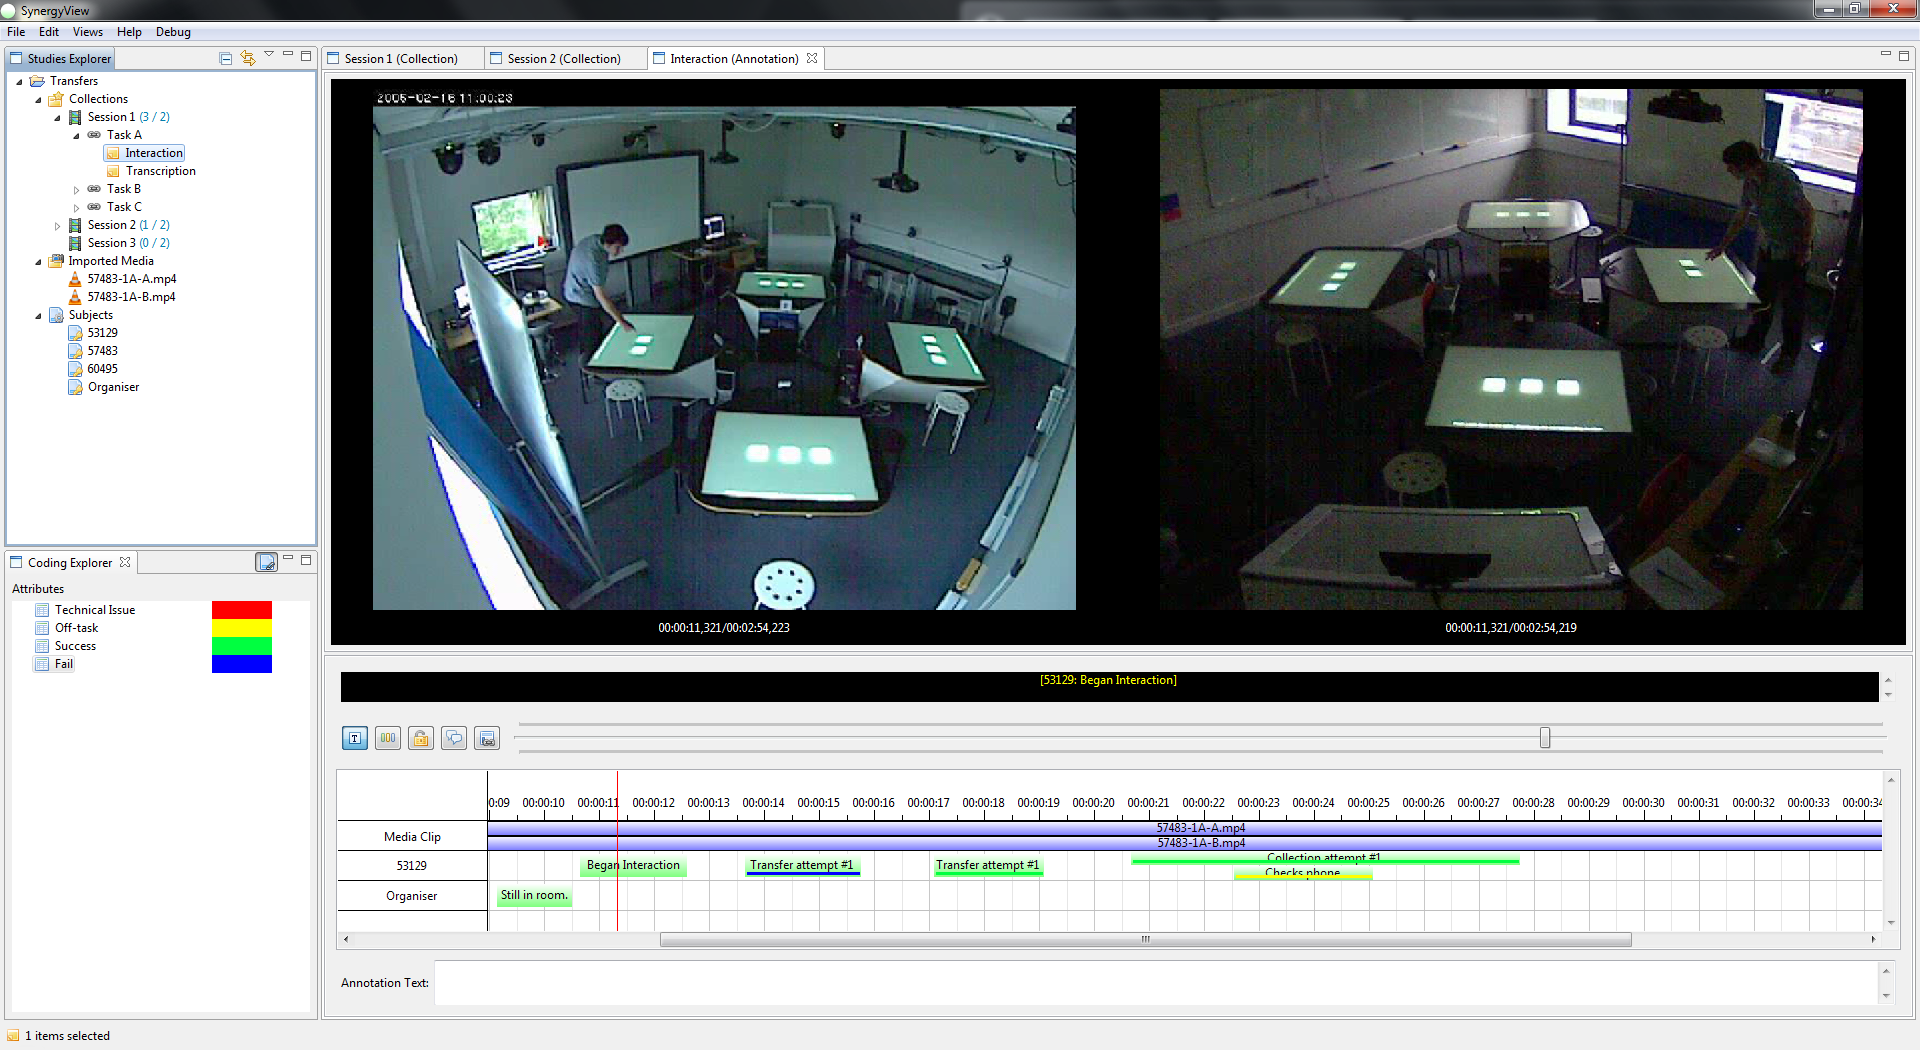
\includegraphics[width=0.75\textwidth]{figures/synergyviewexample.png}
   \caption{The SynergyView video time-line analysis tool in use.}
   \label{fig:SynergyviewExample}
\end{figure}

SynergyView is a time-line analysis tool where multiple videos can be annotated together over time with each annotation being tagged with a wealth of information (such as the subjects in the video they relate to or a type of recurring event seen in the trial). % refs DOI: 10.5281/zenodo.54566
Information on these annotations, such as their frequency, total times and average times can then be exported in a crosstab format for analysis.
The intention is to use SynergyView to annotate the videos from both groups in the study together (once synced).
As multiple sessions took place during the study where different groups of students participated there will be several sets of videos to annotate together.
The resulting crosstabs of information relating each of the sessions can then be collated and analysed as one large data-source.

This quantitative data, in addition to other more qualitative observations made during the sessions and from the videos, should provide some insights into the use osf this study’s configuration of technologies in the classroom.


\section{Lessons Learnt}

% Applying findings and solutions going forward

\subsection{Future Work}

With the changes to the framework made as part of this study, SynergyNet is now well suited for use across the internet where a VPN is set up appropriately.
This will allow for the tables used in this study to be re-deployed anywhere where there is an acceptable 3G/4G signal or with an alternate network connection where the network is configured appropriately.
This will enable for further studies using the framework and the tables used in this study at separate sites.
These further studies may involve following up any discoveries uncovered as part of this study’s data-analysis.

\subsection{Summary} % Maybe not such an obvious title

% Summary of Innovations and theoretical contributions

% BibTeX
\bibliographystyle{ieeetr}
\bibliography{jors2016}

\end{document}
